\newpage
\subsection{General purpose client library implementation}
\label{sec:java_library}

\subsubsection{The technology used}
This section will define a client side of embedded service application.
JSON-RPC messages are used as the main application protocol.
Client part should also support all these features that server offers.

\autoref{fig:rpc_call} showed the main architecture of RPC.
RPC client   application usually consists of two modules: client application code
and client RPC stub, that communicates with remote server.
Client calls usual methods on a stub and the code in a stub handles all
the communication magic, it sends requests, receives responses, serialize and
diserialize data objects.

There were already some examples of a small RPC application (see listings
\ref{lst:rpc_server_python_example} and
\ref{lst:rpc_client_python_example})
Our system requirements and environment does not allow to use Python programming
language.
The client application in this work is written for Google Android smartphone
platform, which has a \gls{JVM} virtual machine inside, and the Java programming
language is used.

Java is very popular programming language which is based on \textit{"Write
once, run anywhere"} philosophy. This means a programmer can develop code on a
PC and can expect it to run on any Java enabled hardware, from small embedded systems
to huge server mainframes. 
This is quite mature programming language with lots of libraries and already
written code that solves different problems. For example, see a list Java tools
for JSON at \url{http://www.json.org/}.

Android system uses Java as one of the main programming language. 
Most programs for android are written using Java and Google provides good
Android development tools for Java programming language.
Android client application will be covered in the next section, while this one will describe the client
stub library which is written in Java. 
This code can be executed on every hardware that is supported by Java virtual
machines. Application architecture in this projects is based on the ideas of
extensibility and portability and therefore Java is a good choice to start.

I have implemented an universal library for the RPC communication with the
previously described embedded service. That library is easy to add to any Java
project and start to develop a new control application. 
It can be extended to add some required funtionality.
 
\subsubsection{Library structure}

The library interface should be identical to a service interface description
or service contract. The JSON service descriptor from the
\autoref{sec:appendix_service_contracts} has enough information to create a
binding library to that embedded service.

This client code can be realized in two different ways: static and dynamic binding.
The library described here, is a static binding library, because it has an already 
defined interface class and client methods are known at the compile time.

Dynamic libraries can determine available server methods at the runtime. Client
library may connect to a server and receives a list of operations. For example JSON
service contract that is used in this work, can be obtained and parsed at the runtime. Dynamic proxy
class can be created from received list of methods and methods can be called
only by a name without the compile time checking. Client may know only a method
name or a part of that name and decide while application is running, which
methods to call. Domain keywords for Java are: \textit{reflection}, \textit{dynamic proxy
class}, \textit{duck typing}. 
The Python example above uses this approach and
you can retrieve list of available methods from server by calling
\texttt{listMethods()} on a \texttt{ServerProxy} object. 
This technique is more suitable for dynamically typed programming languages. 

I preferred to make more robust and simple solution. I created a Java
interface class with all methods that server has. 
The definition of the main interface classes in the library is provided below.

\begin{listing}[H]
\begin{minted}[frame=lines,
               framesep=2mm]{java}
public interface Service {

    // connect methods
    void connect(Reader inputReader, Writer outputWriter);
    boolean isConnected();
    void disconnect();

    public void start();
    public void stop();
    public boolean isRunning();

    boolean addListener(RPCServiceListener listener);
    boolean removeListener(RPCServiceListener listener);

    void setTimeoutMs(long timeoutMs);
    long getTimeoutMs();

    void setRequestProcessor(RequestProcessor requestProcessor);
    RequestProcessor getRequestProcessorByType(
	    Class requestProcessorClass,
	    Object... params);
}               
               
public interface CoffeeMachineService extends Service {
    ServiceContract getServiceContract();
    
    Map<String, Object> getInfo();
    
    // products
    List<Product> getProducts();
    Product.Status orderProduct(int productId);
    Product.Status cancelProduct(int productId);
    Product.Status getProductStatus(int productId);
}
\end{minted}
\caption{RPC client main interface class}
\label{lst:rpc_client_interface_class}
\end{listing}

Some object oriented design techniques are used here to get a more abstract code. 
\texttt{CoffeeMachineService}  extends another
interface \texttt{Service}, which has method that are common to every RPC
service.
\texttt{CoffeeMachineService} interface contains only coffee machine related methods and
inherits other methods from the parent class.

Client can use these classes in the application code and does not need to know
the implementation details. To start using it client needs to create an instance
of \texttt{JsonRpcCoffeeMachineService} ( the implementation of
\texttt{CoffeeMachineService} interface), connect it to \texttt{Reader} and \texttt{Writer} stream objects and after that  user can call RPC methods.

\paragraph{Character encoding} ~\\
Java programming language has the abstraction of \texttt{Reader} and
\texttt{Writer}. These are character stream interfaces that allow to write or
read characters to/from underlying information sources. JSON-RPC is a text
based protocol and we only need to handle character data in our application, but
not binary data.\texttt{Reader} and \texttt{Writer} are parents of
\texttt{InputStreamReader} and \texttt{OutputStreamWriter}, which are bridge
from byte streams to character streams. They transfer bytes to characters and
back using a specified character set\footnote{the mapping between characters and sequences of bytes}.
JVM internally stores characters as 16-bit Unicode variables, but in other
systems character can be:  an US-ASCII seven-bit value, UTF-8 multi-byte
encoding, Extended Binary Coded Decimal Interchange Code (EBCDIC) 8-bit
character encoding and others. Character encoding needs to be specified for
\texttt{InputStreamReader} and \texttt{OutputStreamWriter} in order to convert
data properly. We cannot use byte streams in our library because we cannot
predict in which encoding character data will be received from the data byte
source. It might happen that some byte will have different meaning from what we
expect. Therefore we use an abstraction of \texttt{Reader} and
\texttt{Writer} here.

Client of our library should receive an \texttt{InputStream}  object (operates
with byte streams) from somewhere, provide valid character encoding and create
an \texttt{InputStreamReader} from \texttt{InputStream}, and pass it to
\texttt{connect()} method of the RPC library. The source of an
\texttt{InputStream} may be the array of bytes in the memory, a file on the
disk, a network socket or even String objects. In general words, client should
decide where from data bytes should come, where they need to be written, and
wrap these bytes into character streams.

\paragraph{Message encoding} ~\\

This library assumes that received characters are encoded using
netstrings\footnote{ \texttt{<LENGTH>:<DATA>,} format, for more details see
\autoref{sec:netstrings} } message encoding.
\texttt{MessageReader} class in the library has the implementation of similar finite
state machine parsing algorithm, that was used in the embedded server implementation.
It reads the netstrings encoded messages, extracts the data from them and sends extracted characters to
\texttt{MessageHandler} for processing.


The \texttt{MessageWriter} class composes a valid netstring message and  uses the provided
by a client \texttt{Writer} object to write that message to the destination.
\texttt{MessageWriter} receives JSON  objects,converts them into a String data, wraps them
in a netstring message and sends this character data to the destination.

\paragraph{JSON serialization and the JSON-RPC} ~\\

This JSON-RPC client is based on the \texttt{jsonrpc2-base} library from
Vladimir Dzhuvinov (\url{http://software.dzhuvinov.com}).
This library provides a ready classes for handling JSON-RPC requests and
responses.
\autoref{tbl:jsonrpc2-base_methods} shows the entire lifecycle of a RPC call.



\begin{longtabu} to \linewidth {|p{1cm}|p{1.5cm}|X|p{8cm}|}
 	\caption{jsonrpc2-base library RPC methods \cite{jsonrpc2-base}}
	\label{tbl:jsonrpc2-base_methods} 	 	
\hline 
\multicolumn{1}{|l|}{\textbf{Step}} & 
\multicolumn{1}{l|}{\textbf{Side}} &
\multicolumn{1}{l|}{\textbf{Action}} &  
\multicolumn{1}{l|}{\textbf{Used methods}} \\ 
\hline 
\endfirsthead

\multicolumn{4}{l}%
{{\bfseries \tablename\ \thetable{} -- continued from previous page}} \\
\hline 
\multicolumn{1}{|l|}{\textbf{Step}} & 
\multicolumn{1}{l|}{\textbf{Side}} &
\multicolumn{1}{l|}{\textbf{Action}} &  
\multicolumn{1}{l|}{\textbf{Used methods}} \\ 
\hline 
\endhead

\hline \multicolumn{4}{|r|}{{Continued on next page}} \\ \hline
\endfoot

% \hline \hline
\endlastfoot

		1 &
		Client &
		Create a new request &
		\texttt{JSONRPC2Request()}	
		
		\tabularnewline
		\hline
		2 &
		Client &
		Serialize request to string and send &
		\texttt{JSONRPC2Request.toString()}	
		
		\tabularnewline
		\hline
		3 &
		Server &
		Parse received string back to request object &
		\texttt{JSONRPC2Request.parse()}
		
		\tabularnewline
		\hline
		4 &
		Server &
		Get the request data &
		\texttt{JSONRPC2Request.getMethod()}\newline
		\texttt{JSONRPC2Request.getParamsType()}\newline
		\texttt{JSONRPC2Request.getPositionalParams()}\newline
		\texttt{JSONRPC2Request.getNamedParams()}\newline
		\texttt{JSONRPC2Request.getID()}\newline
		
		\tabularnewline
		\hline
		5 &
		Server &
		Create a response &
		\texttt{JSONRPC2Response()}
		
		\tabularnewline
		\hline
		6 &
		Server &
		Serialise response to string and send back &
		\texttt{JSONRPC2Response.toString()}
		
		\tabularnewline
		\hline
		7 &
		Client &
		Parse received string back to response object &
		\texttt{JSONRPC2Response.parse()}
			
		\tabularnewline
		\hline
		8 &
		Client &
		Check the response for success, get the result/error &
		\texttt{JSONRPC2Response.indicatesSuccess()}\newline
		\texttt{JSONRPC2Response.getResult()}\newline
		\texttt{JSONRPC2Response.getError()}\newline

		
		\tabularnewline
		\hline
	%\end{tabularx} 

\end{longtabu}

\texttt{jsonrpc2-base} is able to serialize Java data types to JSON objects
Listing \ref{lst:jsonrpc2-base_serialization} shows how RPC request object is
created from the standard Java data types and \autoref{tbl:json_java_mapping}
shows how JSON to JAVA mappings are done.

\begin{listing}[H]
\begin{minted}[frame=lines,
               framesep=2mm]{java}
// The remote method to call
String method = "makePayment";

// The required named parameters to pass
Map<String,Object> params = new HashMap<String,Object>();
params.put("recipient", "Penny Adams");
params.put("amount", 175.05);

// The mandatory request ID
String id = "req-001";

// Create a new JSON-RPC 2.0 request
JSONRPC2Request reqOut = new JSONRPC2Request(method, params, id);

// Serialize the request to a JSON-encoded string
String jsonString = reqOut.toString();

// jsonString can now be dispatched to the server...
\end{minted}
\caption{RPC request creating from Java standard data types \cite{jsonrpc2-base}}
\label{lst:jsonrpc2-base_serialization}
\end{listing}


\begin{table}[h]
	\centering	
	\caption{{JSON} \ding{214} {Java} data type mapping in
	\texttt{jsonrpc2-base} library \cite{jsonrpc2-base}}
	\label{tbl:json_java_mapping}
	\begin{tabularx}{0.5\textwidth}{|X|X|}
		\hline
		\textbf{JSON} & \textbf{Java} 	 	\\ \hline	    
		true or false & java.lang.Boolean 	\\ \hline	    
		number & java.lang.Number		 	\\ \hline
	   	string & java.lang.String		 	\\ \hline		
		array & java.util.List		 	\\ \hline
		object & java.util.Map			 	\\ \hline
		null & null		 	\\ \hline			  
	\end{tabularx} 

\end{table}

\paragraph{Data flow} ~\\

This paragraph describes the client stub library RPC call in details. 
Although \texttt{jsonrpc2-base} has classes for handling JSON-RPC message
objects, it does not provide any client functionality. 
We need to write a request handling logic to support the communication with
hardware embedded service.

When client of our library calls any method on \texttt{CoffeeMachineService}
class this method starts to prepare a new request. Service interface
implementation add necessary parameters to RPC request (name, method
parameters, an id), and sends it to request processor.

The whole RPC call process visualized at the \autoref{fig:rpc_call_java} 


\begin{sidewaysfigure}
\centering
\scalebox{0.4}
{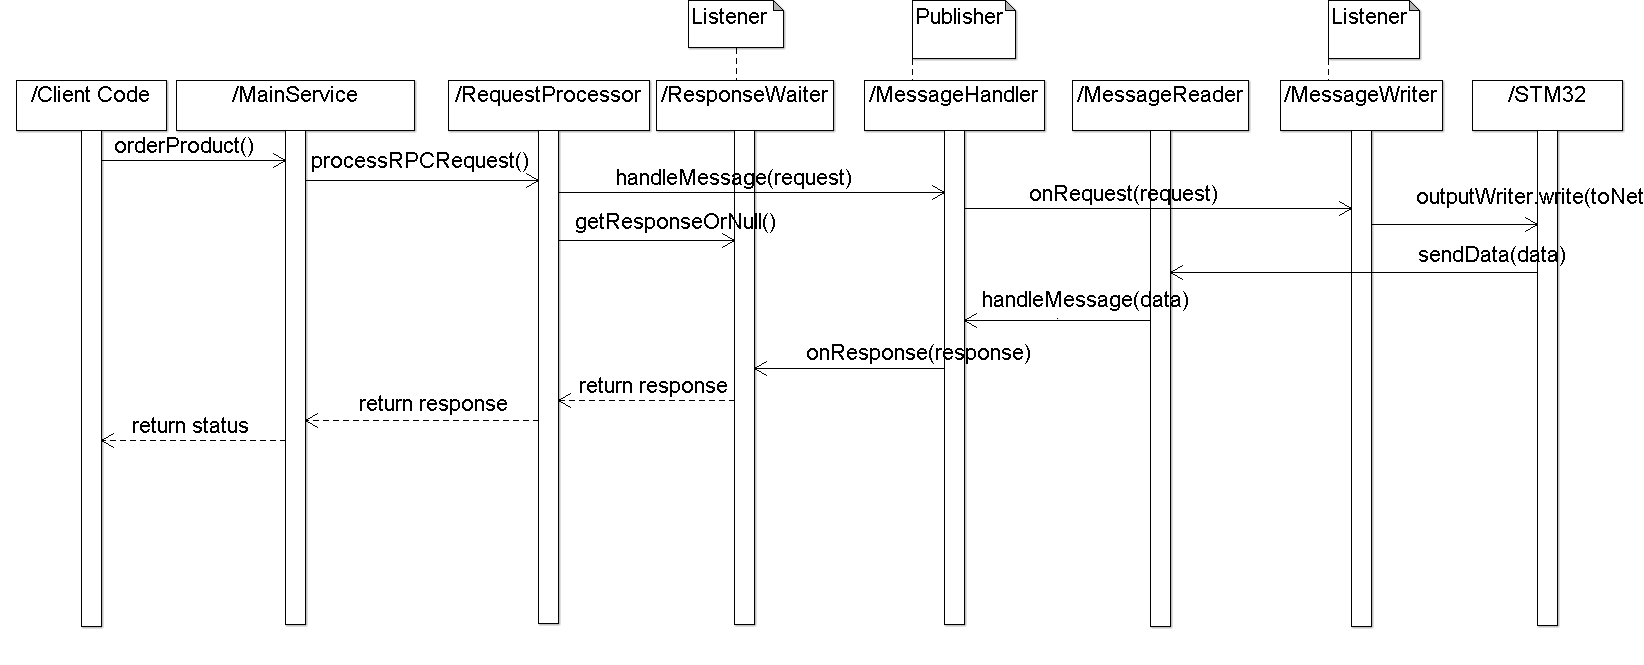
\includegraphics{../images/implementation/java_flow_diagram.png}}
\caption{RPC call in the client stub library}
\label{fig:rpc_call_java}
\end{sidewaysfigure}

\texttt{RequestProcessor} is a simple object with a ~\texttt{Object
processRequest(Object request)} method which encapsulated request processing
logic. Strategy design pattern is implemented here. 
Each request can be processed in a many various ways.
Some methods  have slow execution  on the server and require bigger timeout time
on the client side. Another methods could fail and additional error handling
logic is required. This design methods help to define different  
request handling strategies and apply them at the runtime.
For example the \texttt{getProducts()}  method has very short response time,
because it does not trigger any events on the coffee machine.
Proxy device just returns a list of products from memory storage. 
Another method, the \texttt{orderProduct()}, needs additional communication and
verification of parameters. 
These two methods may have two different algorithms of processing client RPC
request, while programming interface needs to stay fixed.

There is only one strategy for the \texttt{RequestProcessor} implemented yet.
This processor sends a request to a message handler only ones and starts to wait
for a response from a \texttt{RequestWaiter} help class.
After some timeout it returns the result or a \texttt{null} value if there was
not  any response received.

Message writer module of the client stub implements the
\texttt{RPCServiceListener} (pay attention to the 
\texttt{addListener()} and \texttt{removeListener()} methods in listing
\ref{lst:rpc_client_interface_class}) interface. 
This is a \textbf{publish-subscribe mechanism} used in this library for  event
handling.
Service implementation contains a list of service listeners, who are listening
for various RPC messages. 
Listing \ref{lst:event_listener_publisher_interfaces} contains a list o messages that can
be captured by the \texttt{RPCServiceListener}. It also contains a interface of a
class that publishes internal system events.

\begin{listing}[H]
\begin{minted}[frame=lines,
               framesep=2mm]{java}
public interface RPCServiceListener {
    void onRequest(RPCRequest request);
    void onResponse(RPCResponse response);
    void onNotification(RPCNotification notification);
    void onUnknownMessage(String messageText);
}

public interface MessageHandler {
    void handleMessage(String msg);
    void handleMessage(RPCRequest request);
    void handleMessage(RPCNotification notification);
    void handleMessage(RPCResponse response);
}
\end{minted}
\caption{RPC event listener and event publisher interfaces}
\label{lst:event_listener_publisher_interfaces}
\end{listing}

Message writer thread listens for the \texttt{onRequest()} and
\texttt{onNotification()} events. It starts to write request message data to
remote embedded device using the output character \texttt{Writer}  when these
methods are triggered by the request publishers.

System event methods are triggered by a
\texttt{MessageHandler}. This is a small routing class that decides where to put
moving requests, notification, responses and errors according to their types. 
For example, if \texttt{handleMessage(RPCRequest request)} message handler
method is called from somewhere in the code, message handler publishes received
\texttt{RPCRequest} object to all subscribed listeners. 
Message handler calls \texttt{onRequest(RPCRequest request)} method on each
service subscriber and passes new \texttt{RPCRequest} as parameter.

Messages from the the remote device are read by a \texttt{MessageReader} class.
This class reads incoming netstring packets  and passes extracted data
to the \texttt{MessageHandler}. \texttt{MessageHandler} parses incoming JSON 
data and detects that this data type is a JSON-RPC response object. This
Response message becomes published for all listeners including the 
\texttt{ResponeWaiter} help class, who receives message and return it to
\texttt{RequestProcessor}. 


Now the \texttt{RequestProcessor} have received a response it was waiting for
and it can be returned to \texttt{MainService} class. Not the data from the 
response message can be extracted  and remote call result may be returned
to a client code, from where it was initially called.


This is how JSON-RPC messages flow inside service client library.

It might seem quite complicated, but it has lots of advantages. 
Using a publish-subscribe mechanism you might add  multiple event listeners to
the system very easily. 
For example if you need a request logger, you create a class which implements a
\texttt{RPCServiceListener} interface and register it in a main service class 
by calling special methods. Now your logger can listen all RPC
messages and log the information about them.

\paragraph{Conclusion} ~\\

This library can be used in the client application code as the abstract interface of a remote coffee machine.
It makes programming of client code more elegant and easy.
System programmer does not need to develop RPC related code, he can simply use this interface in his projects.
The only necessary step is the connection of a service instance class to the data input and output character streams.
This library uses the netstrings  character data encoding, which is a very simple way how to transfer character data messages.
The whole design is based on the JSON-RPC communication protocol.



